Belle II Flavour tagger is an algorithm that uses \MVA methods to the determine the flavour of a $B$ that is not reconstructed.
In particular, it uses the information of the tag-$B$ meson to infer information about the signal-$B$ meson, in our case the \BtoXsgamma candidate.
The exact procedure is rather complicated and outside of the scope of this thesis, but can be followed up in Ref.\cite{Belle-II:2021zvj}.
The general idea these observables are tested for \epem\ra\qqbar suppression is that a correctly reconstructed $B$-meson should, on average, perform better than a combinatorial \qqbar candidate.
The flavour tagger outputs two distributions: $\mathtt{FT}_{\mathrm{BDT}}$ and $\mathtt{FT}_{\mathrm{NN}}$ which differ by the internal model that the flavour tagger uses (\BDT versus neural network).
The results for \textbf{Test~1} are given in \Cref{fig:Btag_FBDT_qrCombined,fig:Btag_FANN_qrCombined}.
While these variables would offer some separation power, the resulting bias is just above the threshold.

\begin{figure}[htbp!]
    \subcaptionbox{\label{fig:Btag_FBDT_qrCombined}}{
        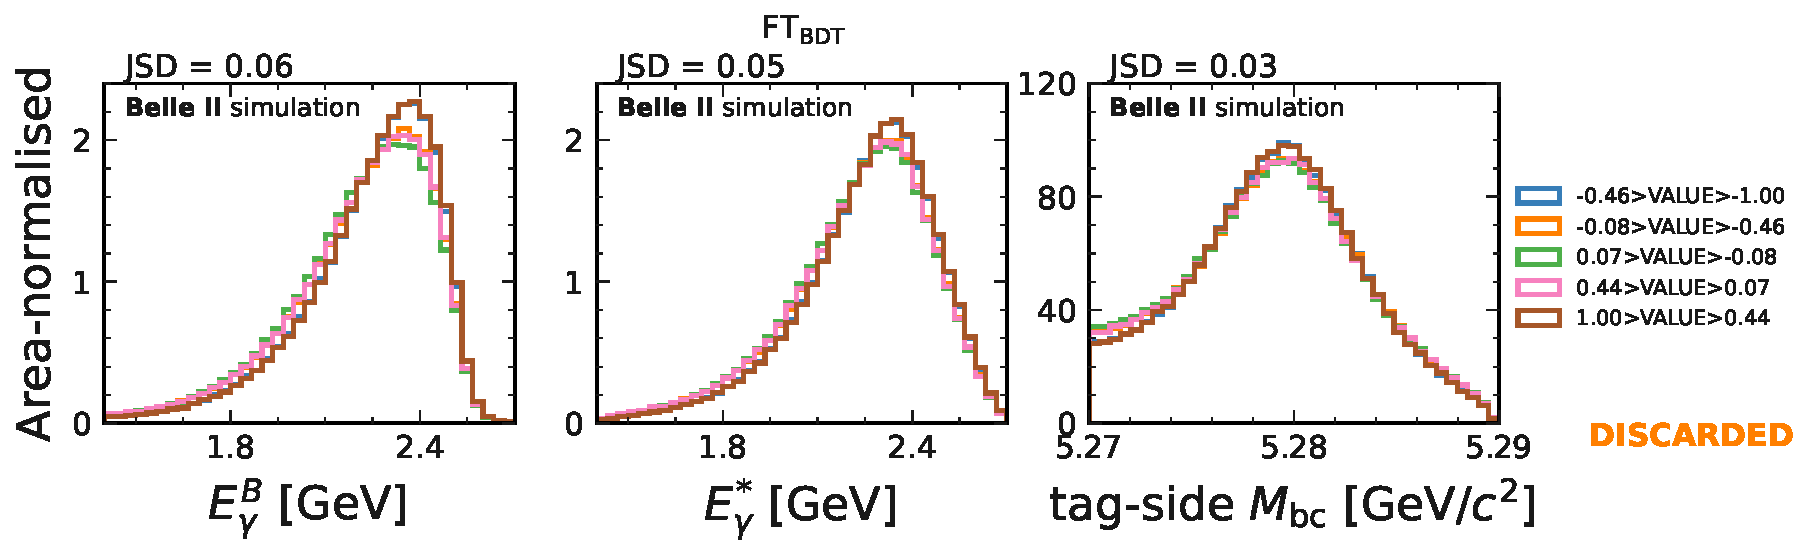
\includegraphics[width=1\textwidth]{figures/appendices/continuum_suppression_features/flavour_tagger_outputs/Btag_FBDT_qrCombined_bias_tested.pdf}

    }
    \subcaptionbox{\label{fig:Btag_FANN_qrCombined}}{
        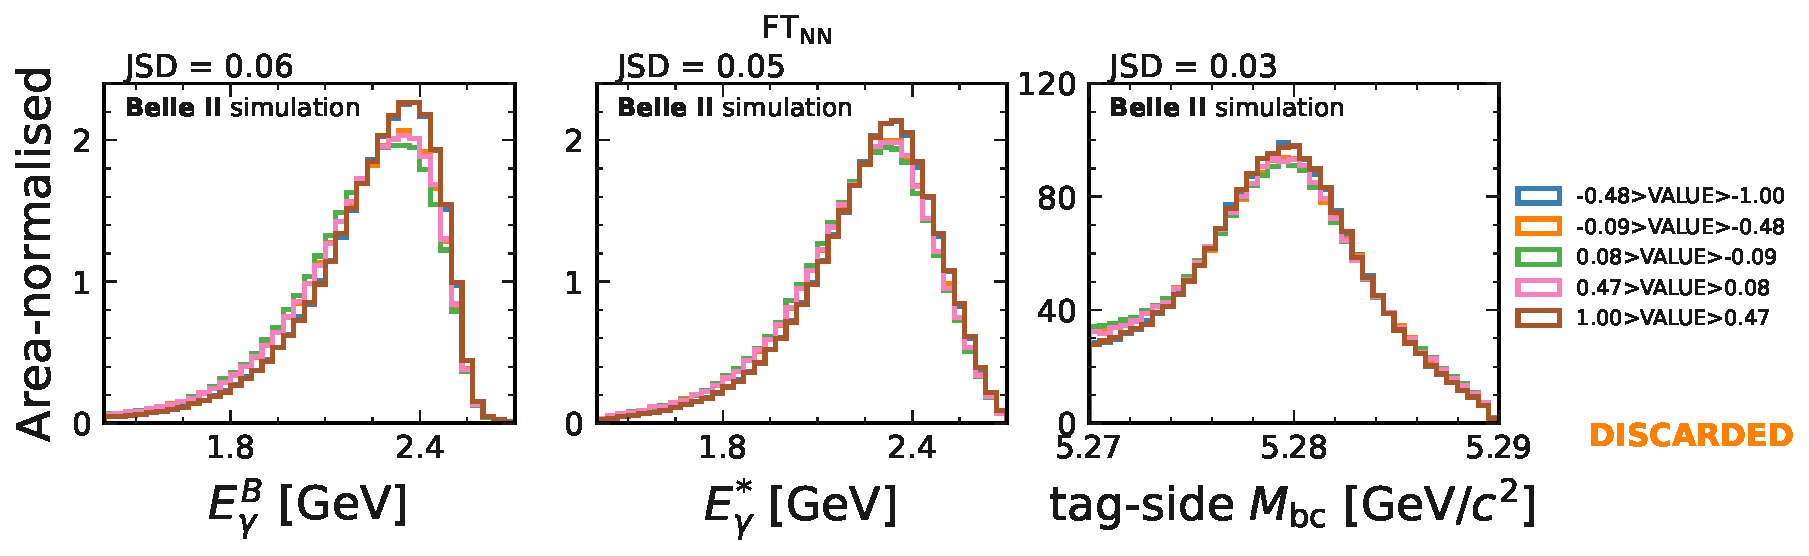
\includegraphics[width=1\textwidth]{figures/appendices/continuum_suppression_features/flavour_tagger_outputs/Btag_FANN_qrCombined_bias_tested.pdf}

    }

    \caption{\label{fig:flavour_tagger_outputs} The bias-test on \EB, \Estar and \Mbc for flavour tagger outputs.
    The test is performed based on \textbf{Test~1} strategy, defined in \Cref{sec:continuum_features}.
    Variable definitions are given in text.}
\end{figure}
